\section{Nef classes in algebraic dimension zero}\label{sec:zero}

A semiample line bundle on a space of algebraic dimension zero is
rationally trivial.  The induction therefore requires a stronger
conclusion in this case: the additional nef class must itself vanish.
The ordinary adjoint decomposition reduces this assertion to a question
about nef line bundles on simple manifolds.  We first carry out that
geometric reduction.  The remaining argument adapts the meromorphic
nonvanishing construction of \cite[Section~6]{K} to a line bundle that
need not be canonical.

\begin{proposition}\label{zero:vanishing}
Let \(n\ge1\).  Assume that the algebraic-dimension-zero assertion of
Theorem~\ref{thm:decomposition} holds in every dimension less than \(n\).
Let \(T\) be a smooth connected compact Kähler \(n\)-fold with
\(a(T)=0\), and let \(B\) be an effective rational simple normal crossing
boundary with coefficients less than one.  If \(K_T+B\) is
pseudo-effective, then every nef rational holomorphic line bundle \(M\)
on \(T\) satisfies \(c_1(M)=0\).
\end{proposition}

For intersections in this Section, a line bundle and its first Chern
class are distinguished when necessary by braces: \(\{H\}=c_1(H)\).
An inequality between real \((1,1)\)-classes is in pseudo-effective
order.  A compact manifold is \emph{simple} if no positive-dimensional
proper compact analytic subvariety passes through a very general point.
Here, as usual, ``very general'' permits deletion of a countable union
of proper analytic subsets.

\subsection{Reduction to a simple symplectic manifold}

The following elementary intersection test lets us use finite covers
without requiring the nef line bundle to descend through them.

\begin{lemma}\label{zero:mass-test}
Let \(V\) be a smooth compact Kähler \(n\)-fold, where \(n\ge1\),
and let \(\gamma\) be a nef
class, and let \(C\) be a nef and big class.  If
\(\gamma\cdot C^{n-1}=0\), then \(\gamma=0\).
In particular, if \(V\) admits a generically finite surjective morphism
to a complex torus of algebraic dimension zero, every nef rational line
class on \(V\) is zero.
\end{lemma}

\begin{proof}
Choose a Kähler class \(\omega\) and \(\varepsilon>0\) such that
\(C-\varepsilon\omega\) is pseudo-effective.  When \(n\ge2\), the
identity
\[
 C^{n-1}-(\varepsilon\omega)^{n-1}
 =(C-\varepsilon\omega)
   \sum_{j=0}^{n-2}C^{n-2-j}(\varepsilon\omega)^j
\]
and nonnegativity of intersections of a pseudo-effective class with
nef classes give
\[
 0=\gamma\cdot C^{n-1}
 \ge \varepsilon^{n-1}\gamma\cdot\omega^{n-1}\ge0.
\]
The same conclusion is immediate when \(n=1\).  A positive current in
\(\gamma\) thus has zero mass, so it vanishes.

For the last assertion, write \(f:V\to A\) for the morphism.  The
pushforward of the nef rational line class is a rational
pseudo-effective \((1,1)\)-class on \(A\).  Averaging a positive current
under translations represents it by a constant semipositive form.  The
kernel of a rational such form is the tangent space of a subtorus; the
induced positive integral form, after clearing denominators, polarizes
the quotient.  Since \(a(A)=0\), this quotient is a point, and hence
\(f_*\gamma=0\).  For a Kähler class \(\eta\) on \(A\), the class
\(C=f^*\eta\) is nef and big and
\[
 \gamma\cdot C^{n-1}=(f_*\gamma)\cdot\eta^{n-1}=0.
\]
Apply the first assertion.
\end{proof}

\begin{lemma}\label{zero:geometric-reduction}
Under the induction hypothesis of Proposition~\ref{zero:vanishing},
it suffices to prove the following assertion: every nef rational line
class on a smooth simple compact Kähler manifold of algebraic dimension
zero carrying a generically nondegenerate holomorphic two-form is zero.
\end{lemma}

\begin{proof}
Apply the ordinary good divisorial decomposition to \(K_T+B\).  On a
smooth modification its semiample part is rationally trivial, because
\(a(T)=0\).  After the klt modification convention of
Section~\ref{sec:preliminaries}, the resulting ordinary adjoint still
equals its rational negative divisor as an actual rational line bundle.
The contraction of a known negative part
\cite[Theorem~2.13 and Proposition~3.8]{K}, with nef part zero, produces
an ordinary compact Kähler klt pair \((T_0,B_0)\) such that
\(K_{T_0}+B_0\qsim0\).

The decomposition theorem of Matsumura--Wang--Wu--Zhang
\cite[Corollary~1.4]{BBYv2} applies to this pair: its nef b-part is zero.
A finite quasi-étale cover of \(T_0\) is a product of a rationally
connected factor, strict Calabi--Yau factors, irreducible holomorphic
symplectic factors, and a torus.  Algebraic dimension is unchanged by
proper generically finite maps and by modifications.  No
positive-dimensional rationally connected factor can occur, since a
Kähler resolution of such a factor is projective by algebraic
connectedness \cite{Campana1981}.  A strict Calabi--Yau factor of
dimension at least three has no holomorphic two-forms.  Extension of
forms for klt spaces \cite{KebekusSchnell2021} gives the same vanishing on a resolution, which is
projective by Kodaira's criterion.  Such factors are also excluded.
Dimension-two factors of Calabi--Yau type are counted among the
symplectic factors.  A resolution of an irreducible symplectic factor
has \(h^{2,0}=1\), generated by a generically nondegenerate form.

Resolve the cover and the maps to \(T\) and to smooth models of all its
factors.  We obtain a smooth compact Kähler manifold \(V\), with the
pulled-back nef line class \(\gamma\), mapping generically finitely to
\(T\) and to a product \(X_1\times\cdots\times X_r\).  If \(r\ge2\),
let \(C\) be the pullback of a sum of Kähler classes from the factors.
For the projection omitting \(X_i\), every component of a smooth general
fiber maps generically finitely to \(X_i\).  This fiber has algebraic
dimension zero and a nonzero top form, obtained by pulling back either
a torus volume form or a power of a symplectic form.  Its canonical class
is therefore pseudo-effective.  Its dimension is less than \(n\), so
the induction hypothesis, with zero boundary, makes the restriction of
\(\gamma\) zero.

Expand \(C^{n-1}\).  A nonzero term has top powers from all factors
except one, where precisely one power is missing.  Integration over the
fibers just considered shows that its pairing with \(\gamma\) is zero.
Thus \(\gamma\cdot C^{n-1}=0\), and Lemma~\ref{zero:mass-test} gives
\(\gamma=0\).  Vanishing descends to \(T\) by push--pull for a
generically finite map.  A single torus factor is covered by the last
assertion of that lemma.

It remains to consider one symplectic factor.  On a smooth model \(X\)
we have \(a(X)=0\) and \(H^0(X,\Omega_X^2)=\C\sigma\), with
\(\sigma\) generically nondegenerate.  There is no dominant meromorphic
fibration from \(X\) to an intermediate-dimensional compact base.
Indeed, on smooth Kähler models such a base has algebraic dimension
zero, hence is nonprojective and has a nonzero holomorphic two-form by
Kodaira's criterion.  Its pullback would be a nonzero degenerate
holomorphic two-form on \(X\), which is impossible.

The minimal-fibration theorem of Campana, in the form
\cite[Theorem~2.3(3) and Corollary~2.5(2)]{COP}, now says that \(X\)
is isotypically semi-simple.  This means that \(X\) and a power
\(S^r\) of a simple manifold have a common generically finite cover;
we may take smooth Kähler models.  If \(r\ge2\), repeat the preceding
product intersection argument.  The smaller-dimensional fibers are
simple: simplicity is preserved by generically finite maps between
spaces of algebraic dimension zero.  Indeed, a covering family of
proper subvarieties upstairs or downstairs gives such a family on the
other space by images or inverse images at points where the map is
finite; the countability of compact cycle components gives the very
general formulation.  They are not uniruled, and hence
their canonical bundles are pseudo-effective by \cite[Theorem~1.1]{Ou}.
The induction hypothesis again applies.  If \(r=1\), the common smooth
cover is simple and carries the pullback of \(\sigma\), a generically
nondegenerate holomorphic two-form.  This is precisely the assertion
stated in the lemma.
\end{proof}

\subsection{Finite correspondences and cotangent slopes}

We next isolate the two geometric properties needed for the
nonvanishing argument.  The first controls subvarieties of a product;
the second controls line subsheaves of cotangent tensors.

\begin{lemma}\label{zero:no-correspondences}
Let \(X\) be a smooth simple compact Kähler manifold of algebraic
dimension zero, carrying a generically nondegenerate holomorphic
two-form.  Suppose that every smooth connected compact Kähler manifold
mapping generically finitely onto \(X\) has irregularity zero.
Through a very general point of \(X^2\), the only positive-dimensional
proper irreducible compact analytic subvarieties are the two factor
slices.
\end{lemma}

\begin{proof}
Fix a generically nondegenerate holomorphic two-form \(\sigma\) on
\(X\).  A moving correspondence would produce a holomorphic one-form
on a fixed finite cover of \(X\).  To see this, we identify its first projection
with a fixed finite cover over a parameter ball, and then contract the
pulled-back two-form in a direction varying the second projection.

For a subvariety through a pair whose coordinates are very general,
simplicity makes each projection image either a point or all of \(X\).
If both projections dominate, their fibers through general points are
either zero-dimensional or the full other factor.  A proper such
subvariety must therefore be a generically finite correspondence.

Suppose these correspondences sweep \(X^2\).  The compact cycle spaces
of a compact Kähler manifold have countably many compact irreducible
components \cite{LiebermanCycles}.  One component must have incidence
image equal to \(X^2\).  Resolve that component and the relevant
incidence component, obtaining a compact Kähler parameter space \(S\),
a smooth incidence space \(Y\), and maps
\[
 h:Y\longrightarrow S,\qquad F_1,F_2:Y\longrightarrow X.
\]
For a general parameter, the fiber is smooth and irreducible, and each
\(F_i\) restricts to a generically finite map.  The map
\((F_1,h):Y\to X\times S\) is generically finite.  Its normal finite
Stein factor is a finite cover of the smooth product.

By purity, the branch locus of this cover is divisorial.  Every branch
component dominating \(S\) has a proper image in \(X\): otherwise its
divisorial fibers over \(S\) would sweep \(X\), contradicting
simplicity.  Compactness of \(S\) makes these images closed analytic
subsets.  Remove the images in \(S\) of the remaining branch components
and take a small ball \(B\) about a general parameter.  There is a fixed
proper analytic subset \(A\subset X\) such that the cover is étale
over \((X\setminus A)\times B\).  Since \(B\) is simply connected,
this étale cover is pulled back from a fixed cover of \(X\setminus A\).
Normalize \(X\) in that cover.  Uniqueness of normal finite extension
then identifies the cover over \(X\times B\) with the product of this
fixed normal cover and \(B\); see
\cite[Exposé~XII, Proposition~5.3 and Theorem~5.4]{SGA1}.

Let \(\widetilde X\) be a smooth Kähler resolution of the fixed cover.
The second projection gives a meromorphic map
\(G:\widetilde X\times B\dashrightarrow X\).  The pullback \(G^*\sigma\)
is a holomorphic two-form: resolve the meromorphic map and descend
holomorphic forms across a modification of a smooth space.  Dominance
of \((F_1,F_2)\) implies that, at suitable general points, the
derivatives of \(G\) in the parameter directions span \(T_X\), while
the derivative along \(\widetilde X\) is an isomorphism.  Choose a
constant tangent vector on \(B\) for which this parameter derivative
is nonzero at such a point.  Contracting \(G^*\sigma\) with that vector
and restricting to \(\widetilde X\times\{t\}\) yields a nonzero global
holomorphic one-form on \(\widetilde X\).  This contradicts the
hypothesis on irregularity.

Each component parametrizing generically finite correspondences thus
has proper incidence image.  Their countable union misses a very
general pair, proving the assertion.
\end{proof}

\begin{lemma}\label{zero:cotangent-slope}
Let \(X\) be a smooth simple compact Kähler manifold of dimension
\(n\ge2\), algebraic dimension zero and irregularity zero, and suppose \(K_X\) is
pseudo-effective.  Let \(\mathscr L\) be a holomorphic line bundle such
that \(L=c_1(\mathscr L)\ge c_1(K_X)\) in pseudo-effective order.
For every nonzero map \(\mathscr H\to\Omega_X^{\otimes k}\), where
\(\mathscr H\) is a line bundle and \(k\ge0\),
\begin{equation}\label{zero:slope-X}
 c_1(\mathscr H)\le kL.
\end{equation}
For every very general \(x\in X\), write
\(a:Y=\operatorname{Bl}_xX\to X\).  Every nonzero line map
\(\mathscr H_Y\to(a^*\Omega_X)^{\otimes k}\) satisfies
\begin{equation}\label{zero:slope-blowup}
 c_1(\mathscr H_Y)\le ka^*L.
\end{equation}
The exceptional set of points can be chosen simultaneously for all
\(\mathscr H_Y\) and \(k\).
\end{lemma}

\begin{proof}
We give the slope argument from \cite[Lemma~6.2]{K}, indicating why it
does not require any hypothesis about canonical sections.  Let
\(\gamma\) belong to the full dual of the pseudo-effective cone.
Ou's convention calls precisely these classes movable, and
Harder--Narasimhan filtrations exist for them
\cite[Definition~4.2 and Lemma~4.3]{Ou}.  If the minimum
\(\gamma\)-slope of \(\Omega_X\) were negative, the first
Harder--Narasimhan subsheaf \(\mathscr T\subset T_X\) would have
positive slope and be semistable.  Tensor slope inequalities make its
bracket into \(T_X/\mathscr T\) zero, so it is a foliation.  Its dual
has negative maximum slope and is non-pseudo-effective.  By
\cite[Theorem~1.4, Lemmas~4.3--4.4 and Proposition~4.5]{Ou}, its leaves have
compact closures given by a meromorphic fibration.  The rank of
\(\mathscr T\) is strictly less than \(\dim X\), since
\(c_1(T_X)\cdot\gamma\le0\).  A general leaf closure contradicts
simplicity.

All Harder--Narasimhan quotient slopes of \(\Omega_X\) are consequently
nonnegative, and its maximum slope is at most
\(c_1(K_X)\cdot\gamma\).  Tensor slopes give
\[
 c_1(\mathscr H)\cdot\gamma
 \le k c_1(K_X)\cdot\gamma\le kL\cdot\gamma.
\]
Separation by the dual cone proves \eqref{zero:slope-X}.

Irregularity zero embeds \(\Pic(X)\) in the countable group
\(H^2(X,\Z)\).  For any vector bundle on \(X\), linearly independent
global sections are generically pointwise independent: the coefficients
expressing one section in a maximal pointwise independent subfamily
are meromorphic functions, hence constants because \(a(X)=0\).
Evaluation is therefore injective outside a proper analytic subset.
Apply this simultaneously to
\(\mathscr H^{-1}\otimes\Omega_X^{\otimes k}\) for all lines
\(\mathscr H\) and all \(k\).

For a point outside the resulting countable exceptional union, write
\(\mathscr H_Y=a^*\mathscr H\otimes\cO_Y(mF)\), where \(F\) is the
exceptional divisor.  A nonzero map as in the statement extends away
from \(F\) to a section on \(X\) by Hartogs.  If \(m>0\), that section
vanishes at \(x\), because \(a_*\cO_Y(-mF)=\mathcal I_x^m\),
contrary to injectivity of evaluation.  Thus \(m\le0\), and
\eqref{zero:slope-X} proves \eqref{zero:slope-blowup}.
\end{proof}

\subsection{Meromorphic nonvanishing from cotangent slope bounds}

The next proposition extracts the line-bundle content of the
construction in \cite[Section~6]{K}.  Its hypotheses deliberately separate
cotangent slopes from the identity of the chosen line bundle.  This is
what permits the application to the sum of the canonical bundle and a
nef line bundle.

\begin{proposition}\label{zero:line-nonvanishing}
Let \(X\) be a smooth simple compact Kähler manifold of dimension
\(n\ge2\), with \(a(X)=0\) and irregularity zero.  Assume that the only
positive-dimensional proper compact irreducible analytic subvarieties
through a very general point of \(X^2\) are its factor slices.
Let \(\mathscr L\) be a holomorphic line bundle with pseudo-effective
class \(L\).  Assume the following line-subsheaf bounds:
\begin{enumerate}
\item For every line bundle \(\mathscr H\), every integer \(k\ge0\),
and every nonzero map \(\mathscr H\to\Omega_X^{\otimes k}\), one has
\(c_1(\mathscr H)\le kL\).
\item Outside a countable union of proper analytic subsets of \(X\),
every point \(x\) has this property: if
\(a:Y=\operatorname{Bl}_xX\to X\), then for every line bundle
\(\mathscr H_Y\), every \(k\ge0\), and every nonzero map
\(\mathscr H_Y\to(a^*\Omega_X)^{\otimes k}\), one has
\(c_1(\mathscr H_Y)\le ka^*L\).
\end{enumerate}
Then some positive power of \(\mathscr L\) has a nonzero meromorphic
section.
\end{proposition}

We prove the proposition by comparing point poles with vanishing along
a diagonal.  Assume, throughout the proof, that no positive power of
\(\mathscr L\) has a nonzero meromorphic section.  A normalized big class
on \(X\) has bounded pole order at a very general point.  On the rank-two projective bundle over \(X^2\) formed from the two
pullbacks of \(\mathscr L\), a class of growing volume produces a
large family of symmetric cotangent tensors.
The diagonal in \(X^2\) forces a large common vanishing order in
their determinant.  The slope inequalities then turn that vanishing into an
impossible point pole on \(X\).

The proof below follows the volume and two-diagonal construction of
\cite[results~6.3--6.10]{K}.  We retain its analytic estimates and give
their proofs along with the determinant calculations, so that the
chosen line bundle enters only through the hypotheses stated above.

\subsubsection{Point pole thresholds}

We will use several standard facts about volumes of real \((1,1)\)-classes.
Our normalization is \(\operatorname{vol}(\alpha)=\int\alpha^e\) for a nef class on an
\(e\)-fold.  Volume is continuous, homogeneous, monotone in
pseudo-effective order, invariant under modification, and its \(e\)-th
root is concave on the big cone.  Analytic Fujita approximation computes
it by Kähler parts on smooth projective modifications.  Here a
\emph{smooth projective modification} means a projective modification
whose source is smooth; the sources used here are compact Kähler
manifolds obtained by resolving coherent analytic ideals.  For a smooth
irreducible divisor \(D\) and a big class \(\alpha\), write
\(\operatorname{vol}_{\,|D}(\alpha)\) for the numerical restricted volume.
It is zero when \(D\) is contained in the non-Kähler locus
\cite[Theorem~1.1]{Vu2023}; otherwise it is
the supremum of the masses on \(D\) of restrictions of Kähler currents
with analytic singularities that are not generically singular on \(D\)
\cite[Lemma~2.7]{CollinsTosatti2018}.  The divisorial derivative and its
continuity on the big cone are
\begin{equation}\label{zero:volume-derivative}
 \frac{\mathrm{d}}{\mathrm{d} u}\operatorname{vol}(\alpha-u\{D\})
   =-e\,\operatorname{vol}_{\,|D}(\alpha-u\{D\});
\end{equation}
see \cite[Theorem~1.1]{Vu2023}.  We apply this formula only on smooth
manifolds while the varying class is big.

Here is a useful precise form of the approximation in the restricted
volume formula.  Resolve the log-ideal singularities of a current
restricted to \(D\).  Its pullback is an effective real divisor plus a
positive residual current with locally bounded potentials.  The latter
dominates a positive multiple of the pulled-back Kähler form.  A current
with locally bounded potentials has zero Lelong numbers, so Demailly
regularization makes its class, after subtracting that multiple, nef
\cite[Theorem~1.1]{DemaillyRegularization1992}.
On a projective modification there is an effective exceptional divisor
whose negative is relatively ample.  Subtracting a sufficiently small
multiple of this divisor from the residual class therefore makes that
class Kähler; add the same multiple to the divisor part.  Round all
divisor coefficients slightly upwards to rational numbers.  Openness of
the Kähler cone preserves the Kähler property.  These changes can be
arbitrarily small in top intersections, which compute the original mass
by the bounded-potential product formula.  Thus we may approximate a
restricted mass by
\begin{equation}\label{zero:rational-fujita}
 h^*(\alpha|_D)=\beta+\{D'\},\qquad
 \beta\ \text{Kähler},\quad D'\ge0\ \text{a rational divisor}.
\end{equation}
Moreover, \(D'\) has at least the log-ideal orders of the original
restriction on every further resolution.  We will use this last
property to turn poles into vanishing conditions.  Only \(D'\) is made
rational; the class \(\beta\) and the horizontal part of \(\alpha\) remain
real.

\begin{lemma}[A point pole bound]\label{zero:pole-threshold}
Let \(W\) be a smooth compact Kähler manifold of dimension \(e\ge2\),
\(\alpha\) a big real \((1,1)\)-class, and \(z\in W\).  Suppose a smooth
projective modification \(\mu:W'\to W\), which is an isomorphism near
\(z\), admits a decomposition
\[
 \mu^*\alpha=K+\{D\},\qquad K\ \text{Kähler},\quad D\ge0,
\]
where \(D\) misses the point \(z'\) over \(z\).  If the ordinary analytic
Seshadri constant \(\epsilon(K,z')\) is at least \(\eta>0\), then, on the
blowup \(b:\widehat W=\operatorname{Bl}_zW\to W\) with exceptional divisor \(G\),
\begin{equation}\label{zero:pole-formula}
 \sup\{u\ge0:b^*\alpha-u\{G\}\ge0\}
 \le \frac{\eta}{2}
     +2^{e-1}\operatorname{vol}(\alpha)\eta^{-(e-1)} .
\end{equation}
\end{lemma}

\begin{proof}
Set \(u_0=\eta/2\).  Blowing up \(z'\), the class
\(K-u_0\{G'\}\) is Kähler.  The Fujita decomposition is unchanged near
\(G'\), so it supplies a Kähler current for
\(\alpha_{u_0}=b^*\alpha-u_0\{G\}\) that is smooth near \(G\).
Its restriction there has class \(u_0c_1(\cO_{\mathbb{P}^{e-1}}(1))\).
The restricted volume is consequently \(u_0^{e-1}\): the current gives
this lower bound, and the volume of the restricted class gives the
opposite bound.

Let \(\tau\) denote the left side of Equation~\eqref{zero:pole-formula}.  The classes
\(\alpha_u=b^*\alpha-u\{G\}\) are big for \(0\le u<\tau\), since
\(\alpha_0\) is big and the pseudo-effective cone is convex.  The
concave function \(f(u)=\operatorname{vol}(\alpha_u)^{1/e}\) satisfies, by
Equation~\eqref{zero:volume-derivative},
\[
 f'(u_0)=-\frac{u_0^{e-1}}{f(u_0)^{e-1}}.
\]
Its tangent line at \(u_0\) must remain positive up to \(\tau\).
Therefore
\[
 \tau\le u_0+\frac{f(u_0)^e}{u_0^{e-1}}
 \le u_0+\frac{\operatorname{vol}(\alpha)}{u_0^{e-1}},
\]
which is Equation~\eqref{zero:pole-formula}.
\end{proof}

Fix a Kähler class \(\omega\) on \(X\).  The class \(L\) is not big:
a big holomorphic line bundle would make \(X\) Moishezon, contrary to
\(a(X)=0\).  For \(t>0\) define
\begin{equation}\label{zero:normalization}
 P=r(L+t\omega),\qquad
 r=\operatorname{vol}(L+t\omega)^{-1/n}.
\end{equation}
Then \(P\) is a big real class, \(\operatorname{vol}(P)=1\), \(L\le P/r\), and
\(r\to\infty\) as \(t\downarrow0\).  Choose a smooth Fujita model
\(\mu:Y_P\to X\) with Kähler part \(P'\) satisfying
\begin{equation}\label{zero:P-prime}
 \mu^*P=P'+\{D_P\},\qquad v:=\int_{Y_P}(P')^n>\frac12.
\end{equation}
At a very general point \(y\) of this model there is no
positive-dimensional proper subvariety: its image would be one through a
very general point of \(X\), and \(y\) avoids the exceptional locus.
The ordinary Seshadri formula for a Kähler class,
\[
 \epsilon(K,y)
  =\inf_{\substack{W\ni y\\ \dim W>0}}
       \left(\frac{\int_W K^{\dim W}}
       {\operatorname{mult}_y W}\right)^{1/\dim W},
\]
therefore gives \(\epsilon(P',y)=v^{1/n}\ge2^{-1/n}\).
This is the ordinary nef/Kähler formula
\cite[Theorem~2.8]{Tosatti2016}; see also
\cite[Equation~(1.5)]{CollinsTosatti2018} and the
Kähler cone criterion of \cite{DemaillyPaun2004}.  We use this ordinary
formula in both applications below.  Lemma~\ref{zero:pole-threshold}, with
\(\operatorname{vol}(P)=1\), now yields a constant \(C_n\) depending only on \(n\)
such that, for a very general \(x\),
\begin{equation}\label{zero:point-bound}
 \tau(P,x):=\sup\{u\ge0:a^*P-u\{F\}\ge0\}\le C_n,
 \qquad a:\operatorname{Bl}_xX\to X.
\end{equation}
Here and below positive constants denoted \(c_n,C_n\) may be decreased or
increased from one occurrence to the next.  They are independent of all
parameters and choices of currents and modifications.

\subsubsection{A projective bundle with controlled volume}

We now produce a class whose volume grows, while its point pole threshold
grows much more slowly.  On \(X^2\), let \(\mathscr L_i\) and \(L_i\)
denote the pullbacks of \(\mathscr L\) and \(L\) from the \(i\)-th factor.
Use the quotient convention and put
\[
 \pi:Z=\mathbb{P}_{X^2}(\mathscr L_1\oplus\mathscr L_2)\longrightarrow X^2,
 \qquad \xi=c_1(\cO_Z(1)),\qquad d=\dim Z=2n+1 .
\]
Thus \(\pi_*\cO_Z(m)=\operatorname{Sym}^m(\mathscr L_1\oplus\mathscr L_2)\) for
\(m\ge0\).  The zero divisor \(A_i\) of
\(\pi^*\mathscr L_i\to\cO_Z(1)\) has class \(\xi-L_i\); it is the
section on which \(\xi\) restricts to \(L_{3-i}\).  In particular
\(\xi=\{A_i\}+L_i\ge0\).

\begin{lemma}\label{zero:subvarieties}
For the projective bundle \(Z\) just defined, the only
positive-dimensional compact irreducible analytic subvarieties through
a very general point are a fiber of \(\pi\), the full inverse images of
the two factor slices, and \(Z\) itself.
\end{lemma}

\begin{proof}
The image of such a subvariety in \(X^2\) is a point, a factor slice,
or all of \(X^2\), by the hypothesis of
Proposition~\ref{zero:line-nonvanishing}.  Generic relative dimension
one gives the full inverse image.  Otherwise, except for a point, the
subvariety is a multisection of the restricted projective line bundle.
On the slice or product \(S\), its divisor line is
\(\cO(k)\otimes\pi^*\mathscr H\), with \(k>0\).  Its homogeneous
equation has coefficients in
\[
 H^0\bigl(S,\mathscr H\otimes
       \mathscr L_1^{\otimes i}\otimes
       \mathscr L_2^{\otimes(k-i)}\bigr),\qquad 0\le i\le k.
\]
A single nonzero monomial cuts out only axes and vertical divisors.
A non-axis multisection therefore has two nonzero coefficients.  Their
quotient is a meromorphic section of a nonzero power of
\(\mathscr L_1\otimes\mathscr L_2^{-1}\).  Restricting to a general
factor slice gives a meromorphic section of a nonzero power of
\(\mathscr L\); inversion makes the power positive if necessary.
This contradicts the standing contrary hypothesis.  The axes
avoid a very general point of \(Z\), proving the lemma.
\end{proof}

Let \(q\) tend to infinity through positive integers.  For each sufficiently
large \(q\), choose \(t=t(q)\) in Equation~\eqref{zero:normalization} so that
\(r=r(q)\ge q^2\), and use the resulting normalized class \(P=P(q)\).
Define the real class and the scale
\begin{equation}\label{zero:M-definition}
 M=P_1+P_2+q\xi,\qquad A_q=q^{1/d}.
\end{equation}

The quantitative goal can now be stated.  On the blowup
\(a:\operatorname{Bl}_xX\to X\) of a very general point, with exceptional
divisor \(F\), we will produce a positive rational scale \(s\) satisfying
\(c_nA_q\le s\le C_nA_q\) and
\[
 2a^*P+(s+2q)a^*L-c_ns\{F\}\ge0.
\]
Since \(L\le P/r\), this would imply
\[
 \frac{c_ns}{2+(s+2q)/r}\le\tau(P,x)\le C_n.
\]
The denominator stays bounded because \(r\ge q^2\), while the numerator
tends to infinity.  To obtain the class inequality, the first diagonal
will produce a subsheaf occupying a fixed positive fraction of a
symmetric cotangent power.  An incidence construction will then force
its determinant to vanish to order proportional to \(s\).  We begin
with the volume that supplies this rank fraction.

\begin{lemma}\label{zero:two-slot-volume}
For these choices, \(M\) is big and
\begin{equation}\label{zero:M-bounds}
 c_nq\le\operatorname{vol}(M)\le C_nq,\qquad
 \tau(M,z):=\sup\{u\ge0:b_z^*M-u\{F_z\}\ge0\}\le C_nA_q
\end{equation}
at a very general point \(z\in Z\), where
\(b_z:\operatorname{Bl}_zZ\to Z\) has exceptional divisor \(F_z\).
\end{lemma}

\begin{proof}
Pull \(Z\) to the Fujita model \(Y_P^2\) from
Equation~\eqref{zero:P-prime}, and put \(H=P'_1+P'_2\) on this pulled-back bundle.
There is a further smooth projective modification
\(\nu:\widehat Z\to\mathbb{P}_{Y_P^2}(\mu^*\mathscr L_1\oplus
\mu^*\mathscr L_2)\) and a Fujita decomposition of the pullback of \(M\)
whose Kähler part is exactly
\begin{equation}\label{zero:exact-K}
 K=\frac12\nu^*H+\Theta ,
\end{equation}
where \(\Theta\) is Kähler and has degree \(q\) on a general vertical
line.  The modification and the divisor part miss that line.

Here is the construction.  It suffices to decompose \(H/2+q\xi\) as
\(\Theta\) plus an effective divisor, clean on a whole general vertical
line.  Since \(\cO(1)\) is relatively ample, a small positive class of
the form \(\delta(\xi+cH)\) is Kähler for some \(c>0\).  Choose
\(\delta>0\) so small that \(\delta<q\) and the remaining horizontal
part of \(H/2\) is Kähler.  Represent the remaining \(\xi\) first as
\(\{A_1\}+L_1\) and then as \(\{A_2\}+L_2\).  Regularize the
pseudo-effective classes \(L_i\) with analytic singularities, paying
their arbitrarily small negative errors from that horizontal Kähler
part.  This gives two Kähler currents in \(H/2+q\xi\), each smooth off
its own axis and a proper horizontal analytic set.  The maximum of
their potentials is locally bounded along an entire general vertical
line, since the two axes are disjoint.  Analytic regularization
preserving a smaller Kähler lower bound
\cite[Theorem~2.1(ii)]{Boucksom2004} gives a Kähler current with
analytic singularities missing that line.  Resolve its singularities
and make the small Kähler adjustment described before
Lemma~\ref{zero:pole-threshold}.  The divisor still misses a general
vertical line, so the residual class \(\Theta\) has degree exactly
\(q\) there.  Adding the other half of \(H\) and the pullbacks of the
divisor parts \(D_P\) gives Equation~\eqref{zero:exact-K}.  Its two
summands are nef, with \(\Theta\) Kähler, so every mixed intersection
used in the following bounds is nonnegative.

At a very general point of \(\widehat Z\), Lemma~\ref{zero:subvarieties}
lists the possible positive-dimensional subvarieties: the vertical line,
the strict transforms of the two full bundles over slices, and
\(\widehat Z\).  They have multiplicity one there.  By
Equation~\eqref{zero:exact-K} and nonnegativity of mixed intersections of nef
classes, their top intersections are respectively bounded below by
\begin{align}
 K\cdot(\text{vertical line})&=q, \notag\\
 \int_{\text{slice}}K^{n+1}
  &\ge \frac{n+1}{2^n}\,qv,\label{zero:K-intersections}\\
 \int_{\widehat Z}K^d
  &\ge \frac{d}{2^{2n}}\binom{2n}{n}\,qv^2. \notag
\end{align}
For example, the middle line is the term containing one factor
\(\Theta\) and \(n\) factors from the varying \(P'\); pushforward of
\(\Theta\) along a general vertical line is \(q\).  The last line is the
term with one \(\Theta\) and \(2n\) horizontal factors.  These
intersections give \(\operatorname{vol}(M)\ge c_nq\).  The ordinary Seshadri formula
and \(q\ge1\) give
\(\epsilon(K,z')\ge c_nq^{1/d}=c_nA_q\) at a very general \(z'\):
each possible dimension is at most \(d\), and every numerator in that
formula is at least \(c_nq\).

For the upper bound, subtract the axis \(A_1\).  For \(0\le u\le q\) put
\[
 M_u=M-u\{A_1\}
     =P_1+P_2+uL_1+(q-u)\xi .
\]
The endpoint \(M_q\) is pulled back from \(X^2\) and has zero volume on
the \(d\)-fold \(Z\).  It is pseudo-effective, and \(M_0\) is big by
the preceding construction, so \(M_u\) is big for \(u<q\).  The
restriction of \(M_u\) to \(A_1\simeq X^2\) is
\[
 (P+uL)_1+(P+(q-u)L)_2.
\]
The restricted volume along \(A_1\) is at most the volume of this
restriction.  For big classes \(\alpha_i\) on manifolds of dimensions
\(e_i\),
\begin{equation}\label{zero:product-volume}
 \operatorname{vol}(\operatorname{pr}_1^*\alpha_1+\operatorname{pr}_2^*\alpha_2)
   =\binom{e_1+e_2}{e_1}\operatorname{vol}(\alpha_1)\operatorname{vol}(\alpha_2).
\end{equation}
One can see this directly from the non-pluripolar product formula
\cite{BEGZ2010}: the
envelope with minimal singularities of a sum on a product is the sum
of the two envelopes, by testing the defining inequality on successive
slices.  Its top product has only the indicated binomial term.  Since
\(L\le P/r\) and \(r\ge q^2\), monotonicity and
Equation~\eqref{zero:product-volume} bound the restriction volume by
\[
 \binom{2n}{n}(1+u/r)^n(1+(q-u)/r)^n\le C_n.
\]
Integrating Equation~\eqref{zero:volume-derivative} from \(0\) to \(q\) gives
\(\operatorname{vol}(M)\le C_nq\).  Finally apply
Lemma~\ref{zero:pole-threshold} with \(e=d\),
\(\eta=c_nA_q\), and \(\operatorname{vol}(M)\le C_nq\).
Both terms on the right of Equation~\eqref{zero:pole-formula} are at most
\(C_nA_q\), since \(A_q^d=q\).  This proves Equation~\eqref{zero:M-bounds}.
\end{proof}

\subsubsection{The first diagonal}

We now use the volume of \(M\) to obtain a high-rank subsheaf of a
symmetric cotangent power on \(Z\).  Distinguish the two copies of \(Z\)
by bracketed indices and
blow up their diagonal:
\[
 b:B=\operatorname{Bl}_{\Delta_Z}(Z\times Z)\longrightarrow Z\times Z,\qquad
 E=b^{-1}(\Delta_Z).
\]
Thus \(E=\mathbb{P}_Z(\Omega_Z)\); its points are normal lines in \(T_Z\).
The dimensions are \(\dim B=2d\) and \(\dim E=2d-1\), and
\(E\to Z\) has relative dimension \(d-1\).
Put \(\zeta=c_1(\cO_E(1))\), so that \(\{E\}|_E=-\zeta\).
For \(s\ge0\) define
\[
 C_s=b^*(M_{[1]}+M_{[2]})-s\{E\},\qquad
 s_{\max}=\sup\{s\ge0:C_s\ge0\}.
\]
The class \(C_0\) is big, so \(s_{\max}>0\) and \(C_s\) is big for
\(0\le s<s_{\max}\).  Restricting a Kähler current with analytic
singularities to the fiber of the first projection at a very general
\(z\in Z\) gives the class \(b_z^*M-s\{F_z\}\).  The current can be
restricted for a general such \(z\), and Lemma~\ref{zero:two-slot-volume}
therefore gives
\begin{equation}\label{zero:smax}
 s_{\max}\le C_nA_q .
\end{equation}
Write \(v_E(s)=\operatorname{vol}_{\,|E}(C_s)\) for
\(0<s<s_{\max}\).  The restriction class is
\begin{equation}\label{zero:restriction-class}
 C_s|_E=2M+s\zeta .
\end{equation}

The intermediate target is a rational \(s\) comparable to \(A_q\) and
a current in \(C_s\) whose restriction to \(E\) has a Kähler part
\[
 h^*(2M+s\zeta)=\beta+\{D'\},\qquad
 h:U\longrightarrow E,
\]
on a smooth projective modification, with \(D'\ge0\) rational, for
which the general fiber volume over \(Z\) satisfies
\[
 w:=\int_{U_z}\beta^{d-1}\ge c_ns^{d-1}.
\]
For such a part, let \(f:U\to Z\) be the natural map and put
\(\Lambda=s h^*\cO_E(1)-\cO_U(D')\).  The direct images
\(\mathcal F_j=f_*\cO_U(j\Lambda)\), for sufficiently divisible \(j\),
are subsheaves of \(\operatorname{Sym}^{js}\Omega_Z\), since \(D'\ge0\).
The direct-image formula below will show that their rank fraction tends
to \(w/s^{d-1}\).  We now prove the bounds needed to obtain this positive
fraction from the total restricted mass.

\subsubsection{A direct-image estimate}

We need to bound a Kähler volume upstairs by a class on the base whose
size can be controlled through determinants.  The base need not be
projective, and the horizontal class is allowed to be real.

The analytic issue is to replace a positive pushforward class by a nef
class on a modified base.  Flattening removes the possible concentration
of mass caused by fibers of excessive dimension.

\begin{lemma}\label{zero:nef-pushforward}
Let \(f:U\to Z_0\) be a surjective projective morphism of smooth connected
compact Kähler manifolds, with \(\dim Z_0=b_0\ge1\) and
\(\dim U=b_0+e\), where \(e\ge1\).  Let \(\beta\) be a Kähler class,
\(w=\int_{U_z}\beta^e\) its general fiber volume, and
\[
 B_0=\frac{f_*\beta^{e+1}}{(e+1)w}.
\]
There are smooth projective modifications \(p:Z'_0\to Z_0\) and
\(q:U'\to U\), and a morphism \(f':U'\to Z'_0\) with
\(pf'=fq\), such that
\[
 B'_0:=\frac{f'_*(q^*\beta)^{e+1}}{(e+1)w}
       =p^*B_0-\{D_0\}
\]
is nef and \(D_0\) is an effective \(p\)-exceptional real divisor.
\end{lemma}

\begin{proof}
Take a smooth projective flattening
modification \(p:Z'_0\to Z_0\), the equidimensional main transform
\(\overline U\) of \(U\times_{Z_0}Z'_0\), and a resolution
\(U'\to\overline U\).  Write \(f':U'\to Z'_0\) and \(q:U'\to U\) for
the maps and \(\beta'=q^*\beta\).  The class
\[
 B'_0=\frac{f'_*(\beta')^{e+1}}{(e+1)w}
\]
is nef.  It is enough to show that the positive pushforward current
representing this class has zero Lelong numbers.  This current can
be computed by integration on the cycle \(\overline U\) of the smooth
form pulled back from \(U\).  At a base point, cover the compact fiber
by finitely many coordinate neighborhoods, each embedded in a product
of base coordinates and ambient coordinates.  In the mass over a base
ball of radius \(\delta\), after wedging with a base Euclidean form to
power \(b_0-1\), the integrand is bounded by a finite sum of projection
volume forms using \(b_0-1\) base coordinates and \(e+1\) generic
linear combinations of all coordinates of the ambient product, including
the remaining base direction.  These projections can be chosen finite on the
neighborhoods: fixing the \(b_0-1\) base coordinates leaves local
dimension at most \(e+1\), by equidimensionality, and generic ambient
coordinates finish a finite projection.  Choose finite proper local
representatives of these projections and then shrink to compact
subneighborhoods.  Their degrees are bounded by the fixed finite
projection degrees; singularities and cycle multiplicities are included
in this bound.  The finite projections form an open dense set of
linear choices.  We can therefore choose a finite collection whose
exterior-coordinate forms span, and hence control, the finitely many
coordinate-minor terms of the integrand.
Change of variables
therefore bounds each integral by
\(O(\delta^{2(b_0-1)})\) times the measure of the remaining coordinate
range.  On each compact subneighborhood these ranges, taken over closed
base balls, are nested compact sets whose intersection is the image of
the central fiber.  That image has measure zero in the \(e+1\) coordinates,
because the fiber has dimension \(e\).  Continuity of finite measure from
above shows that the range measures tend to zero.  Thus the
mass is
\[
 o\bigl(\delta^{2(b_0-1)}\bigr).
\]
This also covers \(b_0=1\), when it asserts absence of an atom.  The
pushforward current has zero Lelong numbers at every point, and
Demailly regularization \cite[Theorem~1.1]{DemaillyRegularization1992}
proves that its class \(B'_0\) is nef.

Pushforward under \(p\) gives \(p_*B'_0=B_0\).  For a modification between
smooth compact Kähler manifolds,
the kernel of pushforward on real Bott--Chern \((1,1)\)-classes is generated
by the classes of its exceptional prime divisors.  Since
\(p_*p^*B_0=B_0\), it follows that \(B'_0-p^*B_0\) is an exceptional real
divisor class.  It is
\(p\)-nef because \(B'_0\) is nef.  Apply relative negativity to this
exceptional real divisor.  Locally over the base, the usual proof for a
projective modification cuts by general hyperplanes to a surface and
uses the negative definite intersection matrix of exceptional curves;
it forces every coefficient of a relatively nef exceptional divisor to
be nonpositive.  Thus
\[
 B'_0=p^*B_0-\{D_0\},\qquad D_0\ge0\ \text{\(p\)-exceptional}.
\]
In particular
\begin{equation}\label{zero:flattened-volume}
 \int_{Z'_0}(B'_0)^{b_0}
  =\operatorname{vol}(B'_0)\le\operatorname{vol}(p^*B_0)=\operatorname{vol}(B_0).
\end{equation}
\end{proof}

The next result combines this nef replacement with the determinant
formula.  It is the quantitative direct-image estimate used in the
construction of symmetric cotangent tensors.

\begin{lemma}\label{zero:direct-image}
Let \(f:U\to Z_0\) be a surjective projective morphism of smooth connected
compact Kähler manifolds, with
\(\dim Z_0=b_0\ge1\) and \(\dim U=b_0+e\), \(e\ge1\).  Suppose
\[
 \beta=f^*G+c_1(\Lambda)
\]
is a Kähler class, where \(G\in H^{1,1}_{\mathrm{BC}}(Z_0,\R)\) and
\(\Lambda\in\Pic(U)\otimes\Q\).  Put
\[
 w=\int_{U_z}\beta^e>0
\]
on a general fiber.  For sufficiently large divisible integers \(j\),
let \(\mathcal F_j=f_*\cO_U(j\Lambda)\) and \(R_j=\operatorname{rk}\mathcal F_j\).
Here \(j\Lambda\) is an actual line bundle and
\(c_1(\mathcal F_j)\) means \(c_1(\det\mathcal F_j)\).  Then
\begin{align}
 R_j&=\frac{w}{e!}j^e+O(j^{e-1}),\label{zero:GRR-rank}\\
 B_0:=G+\lim_j\frac{c_1(\mathcal F_j)}{jR_j}
 &=\frac{f_*\beta^{e+1}}{(e+1)w}\ge0,\label{zero:GRR-base}\\
 \int_U\beta^{b_0+e}
 &\le (e+1)^{b_0}w\,\operatorname{vol}(B_0).\label{zero:mixed-bound}
\end{align}
The limit in Equation~\eqref{zero:GRR-base} is a limit of real Bott--Chern classes.
\end{lemma}

\begin{proof}
The restriction of \(c_1(\Lambda)\) to each fiber is represented by the
restriction of the Kähler form \(\beta\).  The fiberwise criterion for
relative ampleness makes \(\Lambda\) relatively ample after clearing
denominators.  Relative Serre vanishing then kills the higher direct
images for all sufficiently large divisible \(j\).  Analytic
Grothendieck--Riemann--Roch \cite{LevyGRR}, in degrees zero and two, gives
\[
 R_j=\frac{f_*c_1(\Lambda)^e}{e!}j^e+O(j^{e-1}),\qquad
 c_1(\mathcal F_j)
 =\frac{f_*c_1(\Lambda)^{e+1}}{(e+1)!}j^{e+1}+O(j^e).
\]
The degree-zero pushforward is \(w\).  Expanding
\(\beta=f^*G+c_1(\Lambda)\) shows that
\[
 f_*\beta^{e+1}
 =f_*c_1(\Lambda)^{e+1}+(e+1)wG,
\]
because terms with at least two horizontal factors have negative
fiber degree after pushforward.  This proves the equality in
Equation~\eqref{zero:GRR-base}; the cohomological GRR equality is an equality in
Bott--Chern cohomology by the \(\partial\bar\partial\)-lemma on compact
Kähler manifolds.  Pushforward of the positive form
\(\beta^{e+1}\) is a positive closed \((1,1)\)-current, so \(B_0\) is
pseudo-effective.

Apply Lemma~\ref{zero:nef-pushforward} to choose \(p:Z'_0\to Z_0\),
\(q:U'\to U\), and \(f':U'\to Z'_0\), and put \(\beta'=q^*\beta\).
The resulting class \(B'_0\) is nef and satisfies
Equation~\eqref{zero:flattened-volume}.
Choose a Kähler class \(\omega'\) on \(Z'_0\) and put
\(C=B'_0+\varepsilon\omega'\).  For \(0\le k\le b_0\), set
\[
 I_k=\int_{U'}(\beta')^{e+k}(f'^*C)^{b_0-k}.
\]
These are mixed intersections of nef classes.  The first two satisfy
\[
 I_0=w\int_{Z'_0}C^{b_0},\qquad
 I_1=(e+1)w\int_{Z'_0}B'_0C^{b_0-1}
       \le(e+1)w\int_{Z'_0}C^{b_0}.
\]
The mixed nef inequalities make the sequence \(I_k\) log-concave.
Every \(I_k\) is positive: on the dense open where \(q\) is a local
biholomorphism and \(f'\) is a submersion, \(\beta'\) is positive
definite and \(f'^*C\) has rank \(b_0\), so the defining top form
is strictly positive.  The successive ratios are therefore at most
\(I_1/I_0\le e+1\).  Thus
\[
 \int_U\beta^{b_0+e}=I_{b_0}
   \le(e+1)^{b_0}w\int_{Z'_0}C^{b_0}.
\]
Letting \(\varepsilon\downarrow0\) and using
Equation~\eqref{zero:flattened-volume} proves Equation~\eqref{zero:mixed-bound}.
\end{proof}

We will also use the determinant formula without its volume bound.

\begin{corollary}\label{zero:slope-descent}
Let \(Y\) be a smooth compact Kähler manifold and \(\mathscr E\) a
holomorphic vector bundle of rank at least two.  Write
\(\pi_{\mathscr E}:\mathbb{P}_Y(\mathscr E)\to Y\) and
\(\zeta_{\mathscr E}=c_1(\cO_{\mathbb{P}(\mathscr E)}(1))\).
Suppose that a real class \(D\) on \(Y\) satisfies
\[
 c_1(\mathscr H)\le kD
 \quad\text{whenever}\quad
 0\ne\bigl(\mathscr H\longrightarrow\mathscr E^{\otimes k}\bigr)
\]
for a line bundle \(\mathscr H\) and integer \(k\ge0\).
For a real class \(A\) on \(Y\) and a real number \(b\ge0\),
\begin{equation}\label{zero:slope-descent-equation}
 \pi_{\mathscr E}^*A+b\zeta_{\mathscr E}\ge0
 \quad\Longrightarrow\quad A+bD\ge0 .
\end{equation}
\end{corollary}

\begin{proof}
If \(Y\) is a point, both \(A\) and \(D\) vanish and the assertion is
immediate.  Suppose \(\dim Y\ge1\).  Choose a real class \(H_0\) on \(Y\) so that
\(\zeta_{\mathscr E}+\pi_{\mathscr E}^*H_0\) is Kähler; relative
ampleness of \(\cO(1)\) permits such a choice.  Take numbers
\(\delta\downarrow0\) with \(b+\delta>0\) rational.  Adding
\(\delta(\zeta_{\mathscr E}+\pi_{\mathscr E}^*H_0)\) to the
pseudo-effective class in Equation~\eqref{zero:slope-descent-equation} makes it
big.  A Fujita decomposition on a smooth projective modification
\(h:U\to\mathbb{P}_Y(\mathscr E)\), with the divisor coefficients rounded
upwards as in Equation~\eqref{zero:rational-fujita}, has the form
\[
 \beta=f^*(A+\delta H_0)+c_1(\Lambda),\qquad
 \Lambda=(b+\delta)h^*\cO(1)-\cO_U(D')
       \ \text{in }\Pic(U)\otimes\Q,
\]
where \(f=\pi_{\mathscr E}h\), \(\beta\) is Kähler, and \(D'\ge0\)
is rational.  For divisible \(j\),
\[
 f_*\cO_U(j\Lambda)\ \subseteq\
           \operatorname{Sym}^{j(b+\delta)}\mathscr E .
\]
Its determinant of rank \(R_j\) consequently maps into
\(\mathscr E^{\otimes j(b+\delta)R_j}\).  The assumed line inequality
gives
\[
 \frac{c_1(\mathcal F_j)}{jR_j}\le(b+\delta)D.
\]
Lemma~\ref{zero:direct-image} makes
\(A+\delta H_0+\lim c_1(\mathcal F_j)/(jR_j)\) pseudo-effective.
Adding the preceding pseudo-effective difference shows that
\(A+\delta H_0+(b+\delta)D\) is pseudo-effective.  Let
\(\delta\downarrow0\).  This proves the corollary.  In this argument
only \(b+\delta\) and the coefficients of \(D'\) are rational; \(A\),
\(H_0\), and \(D\) remain real classes.
\end{proof}

For the forthcoming application over the \(d\)-fold \(Z\), with fibers
of dimension \(d-1\), Lemma~\ref{zero:direct-image} has a useful concrete
consequence.  Once we prove \(B_0\le C_nM\), the bound
\(\operatorname{vol}(M)\le C_nq\) gives
\[
 \int_U\beta^{2d-1}\le C_nwq.
\]
Thus an upper bound for the normalized determinant class will convert
a lower bound for total mass into a lower bound for the fiber volume
\(w\).  The next calculation supplies the required determinant control.

\subsubsection{Cotangent lines on the projective bundle}

We return to \(Z=\mathbb P_{X^2}(\mathscr L_1\oplus\mathscr L_2)\).
The following calculation is where the chosen line bundle enters the
first determinant estimate.  A line mapping into a cotangent tensor
has nonpositive degree on a general projective-line fiber; the
calculation also controls its horizontal class.

\begin{lemma}\label{zero:cotangent-Z}
Let \(\mathscr H\) be a holomorphic line bundle on \(Z\), and suppose
there is a nonzero map \(\mathscr H\to\Omega_Z^{\otimes k}\), with
\(k\ge0\).  Then
\[
 \mathscr H=\pi^*(\mathscr Q_1\boxtimes\mathscr Q_2)
                   \otimes\cO_Z(\ell)
\]
for lines \(\mathscr Q_i\) on \(X\) and an integer \(\ell\), and
\[
 \ell\le0,\qquad
 c_1(\mathscr Q_1)_1+c_1(\mathscr Q_2)_2
        \le(k-\ell)(L_1+L_2).
\]
\end{lemma}

\begin{proof}
Irregularity zero and Künneth give
\(\Pic(X^2)=\operatorname{pr}_1^*\Pic(X)\oplus
\operatorname{pr}_2^*\Pic(X)\), and the projective-bundle formula for
\(\Pic(Z)\) gives the asserted expression.  Filter the target using
\[
 0\longrightarrow\pi^*\Omega_{X^2}\longrightarrow\Omega_Z
 \longrightarrow\cO_Z(-2)\otimes
        \pi^*(\mathscr L_1\otimes\mathscr L_2)\longrightarrow0.
\]
Choose a nonzero associated graded component.  Suppose it has \(i\)
relative factors and \(k_1,k_2\) cotangent factors from the two copies
of \(X\), so \(k_1+k_2=k-i\).  Its relative degree is \(-2i\).
Pushing to \(X^2\) forces \(m=-2i-\ell\ge0\); hence
\(\ell\le-2i\le0\).  A nonzero monomial in
\(\operatorname{Sym}^m(\mathscr L_1\oplus\mathscr L_2)\), with first
exponent \(m_1\), gives on the two general slices
\[
 c_1(\mathscr Q_1)\le(i+m_1+k_1)L,\qquad
 c_1(\mathscr Q_2)\le(i+m-m_1+k_2)L.
\]
These are exactly the assumed cotangent-line bounds on \(X\), applied
after moving the indicated powers of \(\mathscr L\) to the source.
Each coefficient on the right is at most \(k-\ell\).  Since \(L\ge0\),
pullback and addition prove the claimed bound.
\end{proof}

\subsubsection{Extracting a positive rank fraction}

\begin{lemma}\label{zero:diagonal-mass}
There are constants \(c_n,C_n>0\) such that, for every sufficiently
large \(q\), one can choose a rational number
\[
 c_nA_q\le s\le C_nA_q
\]
and a Kähler current \(T\) in \(C_s\) with analytic singularities,
not generically singular on \(E\), with the following property.  On a
smooth projective modification \(h:U\to E\), its restricted mass has
a rational-divisor approximation
\begin{equation}\label{zero:selected-decomposition}
 h^*(2M+s\zeta)=\beta+\{D'\},
 \qquad \beta\ \text{Kähler},\quad D'\ge0\ \text{rational},
\end{equation}
which retains all log-ideal orders of \(T|_E\).  If
\(f:U\to Z\) is the natural map and
\[
 w=\int_{U_z}\beta^{d-1}
\]
on a general fiber, then
\begin{equation}\label{zero:selected-w}
 w\ge c_ns^{d-1}.
\end{equation}
\end{lemma}

\begin{proof}
First let \(s\) be any rational number in \((0,s_{\max})\) with
\(v_E(s)>0\), and use the approximation in
Equation~\eqref{zero:rational-fujita} for any current used
to compute this restricted volume.  In
Lemma~\ref{zero:direct-image}, the data for Equation~\eqref{zero:restriction-class}
are
\[
 b_0=d,\quad e=d-1,\quad G=2M,\quad
 \Lambda=s h^*\cO_E(1)-\cO_U(D')
           \ \text{in }\Pic(U)\otimes\Q.
\]
For large divisible \(j\), the associated sheaves satisfy
\begin{equation}\label{zero:symmetric-inclusion}
 \mathcal F_j=f_*\cO_U(j\Lambda)
       \subseteq\operatorname{Sym}^{js}\Omega_Z,\qquad
 R_j=\operatorname{rk}\mathcal F_j,\qquad 0<w\le s^{d-1}.
\end{equation}
The inclusion follows by pushing
\(\cO_U(-jD')\subseteq\cO_U\) through \(h\).
For the last inequality restrict the decomposition to a general
\(\mathbb{P}^{d-1}\)-fiber: monotonicity of volume bounds the Kähler volume
there by \(\operatorname{vol}(s\zeta)=s^{d-1}\).

We claim that the class \(B_0\) of Equation~\eqref{zero:GRR-base} satisfies
\begin{equation}\label{zero:B0-bound}
 0\le B_0\le C_nM .
\end{equation}
By Lemma~\ref{zero:cotangent-Z}, write
\[
 \det\mathcal F_j
  =\pi^*(\mathscr Q_{j,1}\boxtimes\mathscr Q_{j,2})
       \otimes\cO_Z(\ell_j),\qquad
 Q_j=c_1(\mathscr Q_{j,1})_1+c_1(\mathscr Q_{j,2})_2.
\]
The determinant of the inclusion in
Equation~\eqref{zero:symmetric-inclusion} gives a nonzero map into
\(\Omega_Z^{\otimes jsR_j}\).  It is defined off codimension two and
extends across that set.  The lemma consequently gives
\begin{equation}\label{zero:determinant-bound-Z}
 \ell_j\le0,\qquad Q_j\le(jsR_j-\ell_j)(L_1+L_2).
\end{equation}

Lemma~\ref{zero:direct-image} supplies a limit of the entire determinant
class divided by \(jR_j\).  The projective-bundle decomposition of
Bott--Chern cohomology gives separate limits \(Q\) and \(\ell\) of
the two displayed components.  Since
\[
 B_0=2(P_1+P_2)+(2q+\ell)\xi+Q\ge0,
\]
testing on a general vertical line gives \(2q+\ell\ge0\).
Equation~\eqref{zero:determinant-bound-Z} gives \(\ell\le0\) and
\(Q\le(s-\ell)(L_1+L_2)\).  Use \(\xi\ge0\), \(-\ell\le2q\),
\(L\le P/r\), \(r\ge q^2\), and \(s\le C_nA_q\le C_nq\).
They give
\[
 B_0\le2(P_1+P_2)+2q\xi+(s+2q)(L_1+L_2)
       \le C_nM,
\]
which proves Equation~\eqref{zero:B0-bound}.

Volume monotonicity, Lemma~\ref{zero:two-slot-volume}, and
Equation~\eqref{zero:mixed-bound} now imply
\begin{equation}\label{zero:restriction-mass-bound}
 \int_U\beta^{2d-1}\le C_nwq,\qquad
 v_E(s)\le C_nq\,s^{d-1}.
\end{equation}
For the second inequality, approximate the mass of each current
arbitrarily closely by \(\beta\) and use \(w\le s^{d-1}\), then take
the supremum over currents.  This proves it for rational \(s\);
continuity of divisorial restricted volume extends it to every
\(s\in(0,s_{\max})\).

At \(s_{\max}\) the class is on the boundary of the pseudo-effective
cone, so its volume is zero.  The product formula in
Equation~\eqref{zero:product-volume}, modification invariance, and the derivative
formula in Equation~\eqref{zero:volume-derivative} yield
\begin{equation}\label{zero:total-diagonal-mass}
 2d\int_0^{s_{\max}}v_E(s)\,\mathrm{d} s
  =\operatorname{vol}(C_0)
  =\binom{2d}{d}\operatorname{vol}(M)^2
  \ge c_nq^2 .
\end{equation}
Choose a fixed small \(\theta_n>0\).  The contribution of
\(0<s<\theta_nA_q\), by Equation~\eqref{zero:restriction-mass-bound}, is at
most \(C_n\theta_n^d q^2\).  Fix \(\theta_n\) small enough that this
is less than half the last lower bound.  The remaining interval has
length at most \(C_nA_q\), by Equation~\eqref{zero:smax}.  Continuity therefore
permits a rational \(s\in[\theta_nA_q,s_{\max})\) such that
\[
 v_E(s)\ge c_nq^2/A_q=c_nqA_q^{d-1}
             \ge c_nq s^{d-1}.
\]
Choose a current with restricted mass at least three quarters of
\(v_E(s)\), and then an approximation as in
Equation~\eqref{zero:selected-decomposition} with
\(\int_U\beta^{2d-1}\ge v_E(s)/2\).  The first inequality of
 Equation~\eqref{zero:restriction-mass-bound} gives
 \(w\ge c_ns^{d-1}\), as claimed.
\end{proof}

For the selected \(s,T,h,\beta,D'\) and \(w\), retain the natural map
\(f:U\to Z\) and put
\[
 \Lambda=s h^*\cO_E(1)-\cO_U(D'),\qquad
 \mathcal F_j=f_*\cO_U(j\Lambda),\qquad R_j=\operatorname{rk}\mathcal F_j,
\]
where \(j\) is sufficiently large and divisible.  Here \(\Lambda\) is a
rational line, and Equation~\eqref{zero:symmetric-inclusion} gives
\(\mathcal F_j\subseteq\operatorname{Sym}^{js}\Omega_Z\).  With \(q\) and these selected
data fixed, Equations~\eqref{zero:GRR-rank} and \eqref{zero:selected-w} give
\begin{equation}\label{zero:selected-rank-fraction}
 \operatorname{rk}\operatorname{Sym}^{js}\Omega_Z=\binom{js+d-1}{d-1},\qquad
 \lim_j\frac{R_j}{\operatorname{rk}\operatorname{Sym}^{js}\Omega_Z}
       =\frac{w}{s^{d-1}}\ge c_n .
\end{equation}
The limit is through divisible integers.  Thus the first diagonal has
produced a subsheaf occupying a fixed positive proportion of the symmetric
power for all sufficiently large divisible \(j\).  The remaining proof
carries this rank bound to a modification of \(Z\) and converts it into a
large common order of vanishing for the determinant map on that model.

\subsubsection{A pole along the incidence}

We next locate a large pole of the selected current \(T\) along a smooth
incidence submanifold of \(B\).  This will impose vanishing conditions on the
symmetric-power subsheaf in Equation~\eqref{zero:symmetric-inclusion}.

Let \(U_0=\pi^{-1}(\Delta_X)\subset Z\), where \(\Delta_X\) is the
diagonal in \(X^2\).  Since
\(\mathscr L_1|_{\Delta_X}=\mathscr L_2|_{\Delta_X}=\mathscr L\), there is a
canonical identification
\[
 U_0=X\times\mathbb{P}^1.
\]
For \(\lambda\in\mathbb{P}^1\) write \(D_\lambda=X\times\{\lambda\}\subset Z\).
Inside \(Z\times Z\) consider
\[
 \mathcal V_0
  =\{((x,x,\lambda),(y,y,\lambda)):x,y\in X,\ \lambda\in\mathbb{P}^1\}
  \simeq X^2\times\mathbb{P}^1.
\]
It meets \(\Delta_Z\) in \(\Delta_X\times\mathbb{P}^1\).  The strict transform
\(V\subset B\) is
\(\operatorname{Bl}_{\Delta_X\times\mathbb{P}^1}\mathcal V_0\); it is smooth, of dimension
\(d=2n+1\).  Its first projection is a smooth family over \(U_0\).
Over \(z=(x,x,\lambda)\) its fiber is
\[
 Y=\operatorname{Bl}_xD_\lambda\simeq\operatorname{Bl}_xX,
\]
and its intersection with \(E\) in that fiber is the projective space
of lines in \(T_zD_\lambda\), inside the projective space of lines in
\(T_zZ\).  These assertions follow either from the blowup of the
section \(y=x\) in this family or from the coordinates used below.

Let \(\rho_V:\operatorname{Bl}_VB\to B\) have exceptional divisor \(G_V\).  Denote
by \(b_V\ge0\) the generic divisorial pole of \(\rho_V^*T\) along
\(G_V\).  Equivalently, it is the generic log-ideal order of \(T\)
along \(V\), with the coefficient of the logarithm included.

\begin{lemma}\label{zero:incidence-pole}
The pole just defined satisfies
\begin{equation}\label{zero:pole-transfer}
 b_V\ge s-C_n .
\end{equation}
\end{lemma}

\begin{proof}
Remove \(b_V[G_V]\) from \(\rho_V^*T\).  Its residual positive current
can be restricted to \(G_V\): for analytic singularities removal of
the generic divisorial pole leaves a potential that is not identically
\(-\infty\) on that divisor.  Choose \(z=(x,x,\lambda)\in U_0\)
general enough for all restrictions and for
Equation~\eqref{zero:slope-blowup} and Lemma~\ref{zero:pole-threshold}.  On the bundle
\[
 G_V|_Y=\mathbb{P}_Y(N^*_{V/B}|_Y),\qquad Y=\operatorname{Bl}_xX,
\]
this restriction is a positive current in the class
\begin{equation}\label{zero:incidence-restriction}
 a^*(2P+qL)-s\{F\}+b_V\zeta_V ,
\end{equation}
where \(\zeta_V=c_1(\cO_{\mathbb{P}(N^*_{V/B}|_Y)}(1))\).
Indeed \(M|_{D_\lambda}=2P+qL\), the first projection to \(Z\) is constant on
\(Y\), and \(E|_Y=F\).  Also \(G_V|_{G_V}=-\zeta_V\), explaining the
positive sign of the last term.

The conormal bundle in Equation~\eqref{zero:incidence-restriction} has exact
sequences
\begin{align}
 0\longrightarrow\cO_Y^{\oplus n}
 &\longrightarrow N^*_{V/B}|_Y
 \longrightarrow a^*N^*_{D_\lambda/Z}\otimes\cO_Y(F)
 \longrightarrow0,\label{zero:incidence-conormal}\\
 0\longrightarrow\Omega_X
 &\longrightarrow N^*_{D_\lambda/Z}
 \longrightarrow\cO_X\longrightarrow0.\label{zero:small-conormal}
\end{align}
The first constant term is the conormal of \(U_0\) in the first copy of
\(Z\), evaluated at \(z\).  For the last term in
Equation~\eqref{zero:incidence-conormal}, the conormal of the strict transform of
\(D_\lambda\) in \(\operatorname{Bl}_zZ\) is
\(a^*N^*_{D_\lambda/Z}\otimes\cO_Y(F)\): in a blowup chart, a normal
coordinate is divided by an exceptional coordinate, giving precisely
the twist by \(F\) for conormals.  Equation~\eqref{zero:small-conormal}
is the conormal sequence for
\(D_\lambda\subset U_0\subset Z\); the diagonal in \(X^2\) has conormal
\(\Omega_X\), and the \(\lambda\)-normal direction is constant on
\(X\).

Filter a \(k\)-fold tensor of \(N^*_{V/B}|_Y\) by these sequences.  A
graded term has the form
\[
 \cO_Y(hF)\otimes(a^*\Omega_X)^{\otimes k'}
          \otimes(\text{a constant vector space}),
 \qquad 0\le k'\le h\le k.
\]
For any nonzero line map into that tensor, take a nonzero graded
component.  Equation~\eqref{zero:slope-blowup} gives
\[
 c_1(\mathscr H_Y)\le h\{F\}+k'a^*L
                 \le k(\{F\}+a^*L),
\]
since both \(\{F\}\) and \(a^*L\) are pseudo-effective.  Apply
Corollary~\ref{zero:slope-descent} to
Equation~\eqref{zero:incidence-restriction}, with
\(D=\{F\}+a^*L\).  We obtain
\begin{equation}\label{zero:incidence-base}
 a^*(2P+(q+b_V)L)-(s-b_V)\{F\}\ge0.
\end{equation}
If \(b_V\ge s\), the conclusion is immediate.  Otherwise
\(b_V<s\le C_nA_q\le C_nq\), and \(L\le P/r\) gives
\[
 \left(2+\frac{q+b_V}{r}\right)a^*P-(s-b_V)\{F\}\ge0.
\]
Use the point bound in Equation~\eqref{zero:point-bound}.  Since \(r\ge q^2\), its
consequence
\[
 s-b_V\le C_n\left(2+\frac{q+b_V}{r}\right)
\]
is bounded by a dimensional constant.  This proves
Equation~\eqref{zero:pole-transfer}.
\end{proof}

\subsubsection{From incidence order to determinant vanishing}

Blow up \(U_0\) in the base of \(E\):
\[
 p_+:Z^+=\operatorname{Bl}_{U_0}Z\longrightarrow Z,\qquad J_+=p_+^{-1}(U_0).
\]
This is the bundle \(Z\) pulled to \(\operatorname{Bl}_{\Delta_X}(X^2)\), since
\(U_0=\pi^{-1}(\Delta_X)\).  In particular \(Z^+\) is smooth.  Put
\[
 E^+=E\times_Z Z^+=\mathbb{P}_{Z^+}(p_+^*\Omega_Z).
\]
Extend the incidence ideal from \(B\) to \(E\), and then to \(E^+\):
\[
 \mathcal J=(\mathcal I_V\cdot\cO_E)\cdot\cO_{E^+}.
\]
The products denote extension of ideals under the indicated maps.
Figure~\ref{zero:two-diagonals} locates \(V\cap E\) and this extension of
the incidence ideal to \(E^+\).

\begin{figure}[ht]
\centering
\begin{minipage}[c]{0.47\linewidth}
\centering
\small
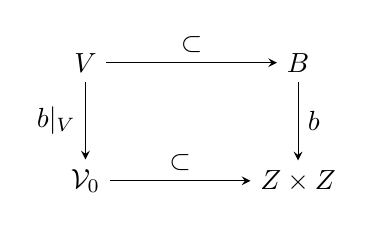
\begin{tikzpicture}[>=stealth, baseline=(current bounding box.center)]
\node (v) at (0,1.5) {$V$};
\node (b) at (2.7,1.5) {$B$};
\node (v0) at (0,0) {$\mathcal V_0$};
\node (zz) at (2.7,0) {$Z\times Z$};
\draw[->] (v)--node[above] {$\subset$} (b);
\draw[->] (v0)--node[above] {$\subset$} (zz);
\draw[->] (v)--node[left] {$b|_V$} (v0);
\draw[->] (b)--node[right] {$b$} (zz);
\end{tikzpicture}
\[
 \begin{gathered}
 V_z=\operatorname{Bl}_xX,\\
 (V\cap E)_z=\mathbb P(T_z^*D_\lambda)
       \subset E_z=\mathbb P(T_z^*Z).
 \end{gathered}
\]
\end{minipage}
\hfill
\begin{minipage}[c]{0.50\linewidth}
\centering
\small
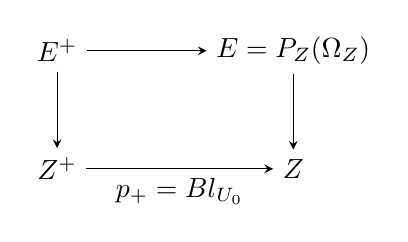
\begin{tikzpicture}[>=stealth, baseline=(current bounding box.center)]
\node (ep) at (0,1.5) {$E^+$};
\node (e) at (3,1.5) {$E=\mathbb P_Z(\Omega_Z)$};
\node (zp) at (0,0) {$Z^+$};
\node (z) at (3,0) {$Z$};
\draw[->] (ep)--(e);
\draw[->] (ep)--(zp);
\draw[->] (e)--(z);
\draw[->] (zp)--node[below] {$p_+=\operatorname{Bl}_{U_0}$} (z);
\end{tikzpicture}
\[
 \begin{gathered}
 J_+=p_+^{-1}(U_0),\qquad U_0=X\times\mathbb P^1,\\
 \mathcal J=(\mathcal I_V\cdot\cO_E)\cdot\cO_{E^+}.
 \end{gathered}
\]
\end{minipage}

\caption{Two geometric constructions used in the determinant estimate.
On the left, the strict transform \(V\subset B\) meets \(E_z\) in the
directions tangent to \(D_\lambda\).  Under the quotient convention,
the displayed projectivized cotangent spaces parametrize tangent lines.
On the right, \(E^+\) is the Cartesian base change
over \(Z^+=\operatorname{Bl}_{U_0}Z\), whose exceptional divisor is \(J_+\).
The restricted incidence ideal extends to \(\mathcal J\) on \(E^+\).
The ensuing local calculation identifies the normal parameter of \(J_+\)
among its generators.}
\label{zero:two-diagonals}
\end{figure}

The next lemma turns the pole bound in
Equation~\eqref{zero:pole-transfer} into a common vanishing order for the
coefficients of each determinant map.

\begin{lemma}\label{zero:determinant-order}
On a smooth projective modification \(h_+:U^+\to E^+\) one can choose
an approximation
\begin{equation}\label{zero:plus-decomposition}
 h_+^*(2p_+^*M+s\zeta)=\beta^++\{D^+\},
 \qquad \beta^+\ \text{Kähler},\quad D^+\ge0\ \text{rational},
\end{equation}
retaining the log-ideal orders of \(T|_E\), such that the general
fiber volume \(w^+\) of \(\beta^+\) over \(Z^+\) satisfies
\(w^+\ge w/2\).  Let \(f_+:U^+\to Z^+\) be the natural map and put
\[
 \Lambda^+=s h_+^*\cO_{E^+}(1)-\cO_{U^+}(D^+),\qquad
 \mathcal F_j^+=(f_+)_*\cO_{U^+}(j\Lambda^+),\qquad
 R_j^+=\operatorname{rk}\mathcal F_j^+ .
\]
For every sufficiently large divisible \(j\), write
\[
 \iota_j:\mathcal F_j^+\hookrightarrow p_+^*\operatorname{Sym}^{js}\Omega_Z,\qquad
 \varphi_j:\det\mathcal F_j^+\longrightarrow
       \bigwedge^{R_j^+}\!\bigl(p_+^*\operatorname{Sym}^{js}\Omega_Z\bigr)
\]
for the inclusion and its nonzero determinant map.  Here
\(\det\mathcal F_j^+=(\bigwedge^{R_j^+}\mathcal F_j^+)^{**}\), and the
determinant map extends across the complement of the locally free locus,
which has codimension at least two.
Localize a coordinate local ring of \(Z^+\) at the height-one prime of
\(J_+\), obtaining a discrete valuation ring \(R\) with uniformizer \(u\).
In local frames over \(R\), define
\[
 h_j=\min\{\operatorname{ord}_u(c):c\text{ is a nonzero coefficient of }\varphi_j\}.
\]
Equivalently, \(h_j\) is the minimum order of the maximal minors of
\(\iota_j\); it is independent of the frames.  If \(\sigma_{J_+}\) is the
canonical section of \(\cO_{Z^+}(J_+)\), then \(\varphi_j\) factors as
\[
 \det\mathcal F_j^+
 \xrightarrow{\ \cdot\sigma_{J_+}^{h_j}\ }
 \det\mathcal F_j^+(h_jJ_+)
 \xrightarrow{\ \widetilde\varphi_j\ }
 \bigwedge^{R_j^+}\!\bigl(p_+^*\operatorname{Sym}^{js}\Omega_Z\bigr),
\]
where \(\widetilde\varphi_j\) is holomorphic.  The common order satisfies
\begin{equation}\label{zero:determinant-order-equation}
 h_j\ge c_n\,jR_j^+s ,
\end{equation}
provided \(q\) is sufficiently large.
\end{lemma}

\begin{proof}
Blow up \(\mathcal J\) and take a common smooth projective resolution
with \(U\to E\) from Equation~\eqref{zero:selected-decomposition}.  Pull back
\(\beta\) and \(D'\).  Subtracting a sufficiently small rational
multiple of an effective exceptional divisor whose negative is
relatively ample makes the pulled-back Kähler class Kähler on this
resolution; add that multiple to the effective part.  Further upward
rational rounding may be
arbitrarily small.  This gives Equation~\eqref{zero:plus-decomposition} with all
original orders retained.  Its general fiber intersection is as close
to \(w\) as desired, so arrange \(w^+\ge w/2\).  Lemma~\ref{zero:direct-image}
and the effective divisor give
\begin{equation}\label{zero:plus-rank}
 \mathcal F_j^+\subseteq p_+^*\operatorname{Sym}^{js}\Omega_Z,\qquad
 R_j^+=\frac{w^+}{(d-1)!}j^{d-1}+O(j^{d-2}).
\end{equation}

We spell out the local order imposed on the polynomials in this
inclusion.  Near \(z=(x,x,\lambda)\), use coordinates
\((\mathbf x,\mathbf a,\lambda)\) on the first \(Z\), where \(\mathbf x\)
and \(\mathbf a\) each have \(n\) components and \(U_0=(\mathbf a=0)\).
Write the second coordinates as
\((\mathbf x+\mathbf h,\mathbf a+\mathbf k,\lambda+\mu)\), with
\(\mathbf h,\mathbf k\) each having \(n\)
components.  Then
\[
 \mathcal V_0=(\mathbf a=\mathbf k=\mu=0),\qquad
 \Delta_Z=(\mathbf h=\mathbf k=\mu=0).
\]
In a blowup chart meeting the lines tangent to \(D_\lambda\), take
\[
 h_1=v,\quad h_i=v\alpha_i\ (2\le i\le n),\quad
 k_i=vy_i\ (1\le i\le n),\quad \mu=vy_{n+1}.
\]
Here \(E=(v=0)\), while the strict transform is
\(V=(a_1=\cdots=a_n=y_1=\cdots=y_{n+1}=0)\).
In particular,
\begin{equation}\label{zero:ideal-before}
 \mathcal I_V|_E=(a_1,\ldots,a_n,y_1,\ldots,y_{n+1}).
\end{equation}
On a chart of the blowup of \(U_0\), write
\(a_1=u\) and \(a_i=u\tau_i\) for \(i\ge2\).  Along the general point
of \(J_+=(u=0)\), the ideal \(\mathcal J\) is exactly
\begin{equation}\label{zero:joint-ideal}
 (u,y_1,\ldots,y_{n+1}).
\end{equation}
Here \(u\) measures vanishing along \(J_+\), while the \(y_i\) measure
transverse fiber directions.  Thus a term of transverse degree \(\ell\)
can contribute at most \(\ell\) to the incidence order; the remaining
order must come from its coefficient in \(u\).  We now make this statement
precise.

Suppose locally that the singularities of \(T\) are
\(c\log|\mathfrak a|+O(1)\), with the logarithmic normalization for
which a divisorial coefficient is \(c\) times the ideal order.  If
\(k=\operatorname{ord}_V(\mathfrak a)\), then \(b_V=ck\).
The normal Taylor coefficients of degree less than \(k\) vanish on a
dense open set of \(V\), hence on \(V\) locally.  Thus
\(\mathfrak a\subseteq\mathcal I_V^k\) also near a general point of
\(V\cap E\).  Restricting to \(E\) and pulling to \(E^+\) gives the
corresponding order in Equation~\eqref{zero:joint-ideal}.  At its general center
the displayed generators are regular coordinates.  If \(H_{\mathcal J}\)
is the exceptional divisor of their blowup, its valuation is the
ordinary ideal-adic order:
\[
 \operatorname{ord}_{H_{\mathcal J}}(g)
  =\max\{k:g\in(u,y_1,\ldots,y_{n+1})^k\}.
\]
The common resolution dominates this blowup.  Pullback preserves the
effective difference between \(D'\) and the resolved log divisor,
and the later adjustments only increase the effective part.  Thus
\(D^+\) has coefficient at least \(b_V\) at this valuation.
Every polynomial image of a section of \(\mathcal F_j^+\) has
integral valuation at least \(\lceil jb_V\rceil\).  Locally bounded
remainders have zero order at this valuation.

There are \(n\) homogeneous coordinates along \(T_zD_\lambda\) and
\(n+1\) transverse homogeneous coordinates in \(T_zZ\).  Denote
these two groups by \(H_1,\ldots,H_n\) and
\(Y_1,\ldots,Y_{n+1}\).  For \(m=js\), a local polynomial in
\(\operatorname{Sym}^m(p_+^*\Omega_Z)\) has the form
\[
 \sum_{|\alpha|+|\gamma|=m}
          c_{\alpha,\gamma}(u)\,H^\alpha Y^\gamma.
\]
Work over the discrete valuation ring \(R\) used to define \(h_j\), choosing
the chart parameter \(u\) as uniformizer, and let \(\kappa\) be its residue
field.  The coefficients \(c_{\alpha,\gamma}\) lie in \(R\).
Equation~\eqref{zero:joint-ideal}
implies, monomial by monomial,
\begin{equation}\label{zero:coefficient-order}
 \operatorname{ord}_u(c_{\alpha,\gamma})
       \ge\max\{0,\lceil jb_V\rceil-|\gamma|\}.
\end{equation}
Indeed, on the chart \(H_1\ne0\), group the dehomogenized polynomial as
\[
 \sum_\gamma
 P_\gamma(H_2/H_1,\ldots,H_n/H_1)(Y/H_1)^\gamma,
 \qquad P_\gamma\in R[H_2/H_1,\ldots,H_n/H_1].
\]
Put \(b_j=\lceil jb_V\rceil\).  At the general center of
\((u,Y/H_1)\), order at least \(b_j\) forces
\(P_\gamma\) to be divisible by \(u^{b_j-|\gamma|}\) whenever
\(|\gamma|<b_j\).  Otherwise its first nonzero reduction would be a
nonzero polynomial over \(\kappa\), which stays nonzero in
\(\kappa(H_2/H_1,\ldots,H_n/H_1)\); in the associated graded ring
it would give a nonzero term of total \((u,Y/H_1)\)-degree less than
\(b_j\).  The transverse monomials there are independent.  Comparing
the internal polynomial coefficients over the base residue field
\(\kappa\) now gives Equation~\eqref{zero:coefficient-order}.

We compare the number of monomials with the rank estimate in
Equation~\eqref{zero:plus-rank}.  The
ambient rank and the number of monomials of transverse degree \(\ell\)
are
\[
 N_m=\binom{m+2n}{2n},\qquad
 N_{m,\ell}=\binom{\ell+n}{n}
             \binom{m-\ell+n-1}{n-1}.
\]
For fixed \(\delta\in(0,1)\), let \(H_m(\delta)\) count the monomials
with \(\ell>(1-\delta)m\).  Summing instead over their internal
degree gives
\[
 H_m(\delta)
 \le \binom{m+n}{n}\binom{\lceil\delta m\rceil+n}{n},\qquad
 \limsup_{m\to\infty}\frac{H_m(\delta)}{N_m}
       \le\binom{2n}{n}\delta^n.
\]
On the other hand, \(w^+\ge w/2\) and
Equation~\eqref{zero:plus-rank} show that the approximation on \(E^+\)
retains at least half the rank fraction in
Equation~\eqref{zero:selected-rank-fraction}:
\[
 \lim_{j\to\infty}\frac{R_j^+}{N_{js}}
       =\frac{w^+}{s^{d-1}}
       \ge\frac{w}{2s^{d-1}}\ge c_n>0.
\]
Fix \(\delta>0\), depending only on \(n\), so small that, for each fixed
\(q\) and its selected data, fewer than \(R_j^+/2\) monomials have transverse
degree greater than \((1-\delta)js\) for all sufficiently large divisible
\(j\).  For each
remaining monomial, Equation~\eqref{zero:coefficient-order} and
Lemma~\ref{zero:incidence-pole} give
\[
 \operatorname{ord}_u(c_{\alpha,\gamma})
   \ge j(s-C_n)-(1-\delta)js
   =j(\delta s-C_n)\ge\frac{\delta js}{2}.
\]
The last inequality holds once \(q\) is large, since
\(s\ge c_nA_q\to\infty\).

Over the same discrete valuation ring \(R\), the torsion-free sheaf
\(\mathcal F_j^+\) becomes a free module of rank \(R_j^+\).  Write its
inclusion into the symmetric power as a matrix with the monomials
as rows.  Every maximal minor uses at least \(R_j^+/2\) of the rows
whose coefficients have order at least \(\delta js/2\).  All maximal
minors therefore have order at least
\(\delta jR_j^+s/4\).  By the definition of \(h_j\), this proves
Equation~\eqref{zero:determinant-order-equation}.  Dividing the determinant
map by \(\sigma_{J_+}^{h_j}\) gives a holomorphic map at every point of
codimension one: the coefficients have the required order along \(J_+\),
and its local equation is a unit away from \(J_+\).  Hartogs' theorem
extends the divided map across the remaining set of codimension at least
two, giving the stated factorization through
\(\det\mathcal F_j^+(h_jJ_+)\).
\end{proof}

\subsubsection{Cancellation on the point blowup}

\begin{proof}[Completion of the proof of Proposition~\ref{zero:line-nonvanishing}]
Fix \(q\) sufficiently large for the preceding lemmas, with its chosen
\(P,s,T\) and modifications.  Choose a very general point \(x\) in the first
factor of \(X^2\).  The slice of \(Z^+\) above \(x\) is
\[
 S=\mathbb{P}_Y(\cO_Y\oplus a^*\mathscr L),\qquad
 a:Y=\operatorname{Bl}_xX\longrightarrow X,
\]
and \(J_+|_S\) is the pullback of \(F\).  We choose \(x\) so that
Equation~\eqref{zero:slope-blowup}, Equation~\eqref{zero:point-bound}, the restrictions of
the currents below, and all determinant maps for divisible \(j\)
can be tested on this slice.  These exclude at most countably many
proper analytic sets and the measure-zero exceptional sets for
current restrictions.

Write the restricted determinant line as
\[
 (\det\mathcal F_j^+)|_S
   =\pi_S^*\mathscr Q_j^+\otimes\cO_S(\ell_j^+),\qquad
 Q_j^+=c_1(\mathscr Q_j^+).
\]
Factoring the common zero of order \(h_j\) from the determinant
map gives a nonzero map whose source on \(S\) is
\[
 \pi_S^*(\mathscr Q_j^+\otimes\cO_Y(h_jF))
                 \otimes\cO_S(\ell_j^+).
\]
The plus sign of \(h_jF\) follows because division of the map by
the local equation of \(J_+^{h_j}\) enlarges its source from
\(\det\mathcal F_j^+\) to
\(\det\mathcal F_j^+\otimes\cO(h_jJ_+)\).
Its target embeds into the \(jsR_j^+\)-fold tensor of the
restriction of \(p_+^*\Omega_Z\).  In particular we use the
cotangent bundle of the original \(Z\), with its restricted
filtration
\[
 0\longrightarrow
 \pi_S^*(\cO_Y^{\oplus n}\oplus a^*\Omega_X)
 \longrightarrow (p_+^*\Omega_Z)|_S
 \longrightarrow
 \cO_S(-2)\otimes\pi_S^*a^*\mathscr L
 \longrightarrow0.
\]
The same homogeneous-monomial calculation as in
Equation~\eqref{zero:determinant-bound-Z}, now applying
Equation~\eqref{zero:slope-blowup} to the second factor of \(X^2\), gives
\begin{equation}\label{zero:determinant-bound-slice}
 \ell_j^+\le0,\qquad
 Q_j^++h_j\{F\}
       \le(jsR_j^+-\ell_j^+)a^*L.
\end{equation}
More explicitly, if the chosen graded term has \(i\) relative
factors, the pushed polynomial has degree
\(-2i-\ell_j^+\ge0\).  Its exponent in \(a^*\mathscr L\), together
with the \(i\) relative factors and the cotangent order from the second
factor of \(X^2\), is at most \(jsR_j^+-\ell_j^+\).  The cotangent
factors from the first factor of \(X^2\) are constant.  This proves the
displayed inequality using
the tensors of \(a^*\Omega_X\), without introducing \(\Omega_Y\)
or \(\Omega_{Z^+}\).

Apply Lemma~\ref{zero:direct-image} to the decomposition in
Equation~\eqref{zero:plus-decomposition}.  Equation~\eqref{zero:GRR-base}
shows that the limits of the restricted determinant components divided by
\(jR_j^+\) exist; denote them by \(Q^+\) and \(\ell^+\).  Divide
Equation~\eqref{zero:determinant-bound-slice} by \(jR_j^+\), use
Equation~\eqref{zero:determinant-order-equation}, and pass to the closed
pseudo-effective cone.  We obtain
\begin{equation}\label{zero:slice-upper}
 \ell^+\le0,\qquad
 Q^++c_ns\{F\}\le(s-\ell^+)a^*L.
\end{equation}
The pseudo-effective class in Equation~\eqref{zero:GRR-base}, restricted to the
very general slice \(S\), is
\begin{equation}\label{zero:slice-psef}
 \pi_S^*(Q^++2a^*P)+(\ell^++2q)\xi\ge0.
\end{equation}
Testing on a general vertical line gives \(\ell^++2q\ge0\).
Let \(A\subset S\) be the axis of
\(\mathbb{P}_Y(\cO_Y\oplus a^*\mathscr L)\) with divisor class \(\{A\}=\xi\).
On \(A\simeq Y\), its normal class is \(\{A\}|_A=\xi|_A=a^*L\ge0\).
Add an arbitrarily small Kähler class to the class in
Equation~\eqref{zero:slice-psef}, and choose a Kähler current with analytic
singularities in the resulting big class.  Remove its generic divisorial
pole along \(A\) and restrict
the residual current to \(A\).  Adding back the removed nonnegative multiple
of \(a^*L\) preserves pseudo-effectivity.  Passing to the limit gives
\begin{equation}\label{zero:slice-lower}
 Q^++2a^*P+(\ell^++2q)a^*L\ge0.
\end{equation}

The slope bound in Equation~\eqref{zero:slice-upper} supplies the
pseudo-effective class \((s-\ell^+)a^*L-Q^+-c_ns\{F\}\).  Adding it to
Equation~\eqref{zero:slice-lower} cancels the entire normalized determinant
class restricted to the axis, \(Q^++\ell^+a^*L\), leaving
\[
 2a^*P+(s+2q)a^*L-c_ns\{F\}\ge0.
\]
Since \(L\le P/r\), the point bound in Equation~\eqref{zero:point-bound} implies
\begin{equation}\label{zero:contradiction}
 \frac{c_ns}{\,2+(s+2q)/r\,}\le C_n.
\end{equation}
The denominator is bounded independently of \(q\), because
\(s\le C_nq^{1/d}\) and \(r\ge q^2\).  The numerator tends to
infinity, because \(s\ge c_nq^{1/d}\).  Equation~\eqref{zero:contradiction}
is impossible for arbitrarily large \(q\).

For each \(q\), the choice of \(t(q)\), the rational \(s\), the current
\(T\), and the modifications precedes the limit in \(j\).  The monomial
cutoff \(\delta\) depends only on \(n\), while the required lower bound for
divisible \(j\) may depend on the fixed data.  We choose the very general
points after those data are fixed.
Thus every simultaneous general-point test above involves at most
countably many conditions, and no bound depends on the point.
The contradiction disproves the contrary hypothesis and proves
Proposition~\ref{zero:line-nonvanishing}.
\end{proof}

\subsection{Vanishing on the simple model}

We now apply Proposition~\ref{zero:line-nonvanishing} to the sum of
the canonical bundle and the nef line bundle whose class we wish to
eliminate.  The remaining use of the ordinary adjoint
decomposition is particularly short: it turns meromorphic
nonvanishing into both signs of pseudo-effectivity.

\begin{proposition}\label{zero:simple-vanishing}
Let \(X\) be a smooth simple compact Kähler manifold of algebraic
dimension zero carrying a generically nondegenerate holomorphic
two-form.  Every nef rational holomorphic line bundle on \(X\) has zero
first Chern class.
\end{proposition}

\begin{proof}
The assertion is immediate for a point.  A positive-dimensional space
of algebraic dimension zero cannot be a curve, so assume \(\dim X\ge2\).
If \(q(X)>0\), its Albanese map is generically finite onto its image,
by simplicity.  Ueno's structure theorem for subvarieties of complex
tori makes this image a translate of a torus: its quotient by the
connected stabilizer is of general type, and positive dimension of that
quotient would contradict algebraic dimension zero \cite{Ueno}.
Lemma~\ref{zero:mass-test} proves the conclusion.

The same argument applies after any smooth generically finite Kähler
cover of \(X\) having positive irregularity.  Such a cover is still
simple and has algebraic dimension zero; vanishing upstairs descends
by push--pull.  We may therefore suppose that every such cover has
irregularity zero.  Lemma~\ref{zero:no-correspondences} then describes
the subvarieties through a very general point of \(X^2\).

Clear denominators and let \(N_0\) be the resulting nef holomorphic line
bundle.  A top wedge of the generically nondegenerate two-form is a
nonzero holomorphic section of \(K_X\).  In particular \(K_X\) is
effective.  Set
\[
 \mathscr L=K_X+N_0,\qquad L=c_1(\mathscr L).
\]
The class \(L\) is pseudo-effective and dominates \(c_1(K_X)\).
Lemma~\ref{zero:cotangent-slope} supplies both slope inequalities.
Every hypothesis of Proposition~\ref{zero:line-nonvanishing} is now
satisfied.  Some positive power of \(K_X+N_0\) therefore has a nonzero
meromorphic section.  Dividing by the corresponding power of a
canonical section shows that \(N_0\), as a rational line bundle, is
represented by a signed divisor.

Resolve its positive and negative parts.  On the resulting smooth
Kähler model write
\[
 N_0\qsim E-G,\qquad E,G\ge0,
\]
with rational coefficients and simple normal crossing union of their
supports; we suppress the pullback notation for \(N_0\).  The canonical
bundle \(K'\) of this model remains effective.  Choose a small rational
\(u>0\) so that both \(uE\) and \(uG\) are klt boundaries.
The ordinary decomposition, Theorem~\ref{pre:ordinary}, applies to
\(K'+uE\) and \(K'+uG\).  On a common higher model, denote their pulled
back classes by \(\alpha_E\) and \(\alpha_G\).  Algebraic dimension zero
makes each semiample part rationally trivial, so that the pulled back
rational lines equal their negative divisors.  Since
\(\alpha_E-\alpha_G=u\{N_0\}\) is nef,
Lemma~\ref{pre:negative}\,(2) gives
\[
 N(\alpha_E)\le N(\alpha_G),\qquad
 u\{N_0\}=\{N(\alpha_E)-N(\alpha_G)\}.
\]
Thus \(-\{N_0\}\) is pseudo-effective, whereas \(\{N_0\}\) is nef.
Pairing both classes with a Kähler power gives zero mass, and hence
\(\{N_0\}=0\).  Pullback injectivity yields the same conclusion on
\(X\).
\end{proof}

\begin{proof}[Proof of Proposition~\ref{zero:vanishing}]
Lemma~\ref{zero:geometric-reduction} reduces the assertion to
Proposition~\ref{zero:simple-vanishing}, which proves it.
In particular, once the induction has reached dimension \(n\), the
ordinary decomposition of \(K_T+B\) also proves the decomposition
assertion of Theorem~\ref{thm:decomposition} in algebraic dimension
zero: adding the nef line changes no Chern class.  Its semiample positive
part is rationally trivial, and its negative part is unchanged.
\end{proof}
